\chapter{Instalación de paquetes y programas en los nodos de Cadejos}
Al realizar una instalación desde cero de un nodo del clúster Cadejos, es necesario instalar una serie de paquetes y realizar ciertas configuraciones para su óptimo uso y funcionamiento. A continuación se listan los paquetes y repositorios que se deben agregar.

\section{Repositorios recomendados}

Para agregar el repositorio EPEL:

\begin{lstlisting} 
rpm -Uvh http://dl.fedoraproject.org/pub/epel/7/x86_64/e/epel-release-7-5.noarch.rpm
\end{lstlisting}

Para habilitar el repositorio REMI:

\begin{lstlisting} 
rpm -Uvh http://rpms.famillecollet.com/enterprise/remi-release-7.rpm
\end{lstlisting}

Con esto listo, procedemos a actualizar el software instalado para luego instalar los programas requeridos \cite{centosrepos}.

\section{Instalación de paquetes esenciales}

Hacemos lo siguiente:

\begin{lstlisting} 
yum update -y && yum upgrade -y
yum install screen a52dec a52dec-devel abrt abrt-addon-ccpp abrt-addon-kerneloops abrt-addon-python abrt-cli abrt-libs abrt-python abrt-tui acl acpid aic94xx-firmware alsa-lib alsa-lib-devel alsa-utils ant antlr apache-tomcat-apis apr apr-util at atk atk-devel atlas atlas-3dnow atlas-3dnow-devel atlas-devel atlas-sse atlas-sse2 atlas-sse2-devel atlas-sse3 atlas-sse3-devel atlas-sse-devel atmel-firmware attr audit audit-libs audit-libs-python augeas-libs authconfig autoconf autofs automake avahi-libs b43-fwcutter b43-openfwwf basesystem bash bc bcel bfa-firmware bind-libs bind-utils binutils bison blacs-common blacs-mpich blacs-mpich-devel blas blas-devel  blktrace bridge-utils bsf btparser busybox byacc bzip2 bzip2-devel bzip2-devel bzip2-libs bzip2-libs ca-certificates cairo cairo-devel cdparanoia-libs celt centos-indexhtml centos-release check check-devel checkpolicy chkconfig cifs-utils cl-asdf classpathx-jaf classpathx-mail cloog-ppl cmake cmake28 cmake-gui common-lisp-controller compat-gcc-34 compat-gcc-34-g77 compat-libf2c-34 ConsoleKit ConsoleKit-libs coreutils coreutils-libs cpio cpp cpuspeed cracklib cracklib-dicts crash crda createrepo cronie cronie-anacron crontabs cryptsetup-luks cryptsetup-luks-libs cscope ctags cups cups-libs curl cvs cyrus-sasl cyrus-sasl-lib cyrus-sasl-plain dash db4 db4-utils dbus dbus-glib dbus-libs dbus-python dejavu-fonts-common dejavu-lgc-sans-fonts dejavu-lgc-sans-mono-fonts dejavu-lgc-serif-fonts dejavu-sans-fonts dejavu-sans-mono-fonts dejavu-serif-fonts deltarpm desktop-file-utils device-mapper device-mapper-event device-mapper-event-libs device-mapper-libs device-mapper-multipath device-mapper-multipath-libs device-mapper-persistent-data dhclient dhcp-common diffstat diffutils dirac-devel dirac-libs dmidecode dmraid dmraid-events docbook-dtds docbook-style-dsssl docbook-style-xsl docbook-utils dosfstools doxygen dracut dracut-kernel e2fsprogs e2fsprogs-libs ed efibootmgr eggdbus eject elfutils elfutils-libelf elfutils-libs enca enchant epel-release ethtool expat faac faac-devel faad2-devel faad2-libs fakeroot fakeroot-libs ffmpeg ffmpeg-compat ffmpeg-devel ffmpeg-libs fftw fftw2 fftw2-devel fftw-devel file file-libs filesystem findutils fipscheck fipscheck-lib firefox flac flex fltk fontconfig fontconfig-devel fontpackages-filesystem fprintd fprintd-pam freeglut freeglut-devel freetype freetype-devel fribidi fuse gamin ganglia ganglia-gmond gawk gcc gcc-c++ gcc-gfortran GConf2 gd gdb gdbm gdk-pixbuf2 gdk-pixbuf2-devel gettext gettext-devel gettext-libs ghc ghc-array ghc-array-devel ghc-base ghc-base-devel ghc-bytestring ghc-bytestring-devel ghc-Cabal ghc-Cabal-devel ghc-compiler ghc-containers ghc-containers-devel ghc-directory ghc-directory-devel ghc-extensible-exceptions ghc-extensible-exceptions-devel ghc-filepath ghc-filepath-devel ghc-ghc ghc-ghc-devel ghc-haskell2010 ghc-haskell2010-devel ghc-haskell98 ghc-haskell98-devel ghc-hpc ghc-hpc-devel ghc-libraries ghc-old-locale ghc-old-locale-devel ghc-old-time ghc-old-time-devel ghc-pretty ghc-pretty-devel ghc-process ghc-process-devel ghc-random ghc-random-devel ghc-template-haskell ghc-template-haskell-devel ghc-time ghc-time-devel ghc-unix ghc-unix-devel ghostscript ghostscript-devel ghostscript-fonts giflib git glew glib2 glib2-devel glibc glibc glibc-common glibc-devel glibc-headers glibc-static glib-networking glpk gmp gmp-devel gnome-keyring gnupg2 gnuplot gnuplot-common gnutls gnutls-devel gpgme gpg-pubkey gpg-pubkey gpg-pubkey gpg-pubkey gpg-pubkey gpm-libs GraphicsMagick GraphicsMagick-c++ GraphicsMagick-doc grep groff grub grubby gsl gsl-devel gsm gsm-devel gstreamer gstreamer-devel gstreamer-ffmpeg gstreamer-plugins-base gstreamer-plugins-base-devel gstreamer-tools gtk2 gtk2-devel gtk-doc gzip hal hal-info hal-libs hamcrest hardinfo hdparm hesiod hicolor-icon-theme hsqldb htop hunspell hwdata hwloc ilmbase ImageMagick ImageMagick-c++ ImageMagick-c++-devel ImageMagick-devel ImageMagick-doc ImageMagick-perl imlib2 imlib2-devel indent infinipath-psm info initscripts intltool iproute iptables iptables-ipv6 iputils ipw2100-firmware ipw2200-firmware irqbalance iscsi-initiator-utils iso-codes ivtv-firmware iw iwl1000-firmware iwl3945-firmware iwl4965-firmware iwl5000-firmware iwl5150-firmware iwl6000-firmware iwl6050-firmware jakarta-commons-codec jakarta-commons-httpclient jakarta-commons-logging jakarta-oro jasper-devel jasper-libs java-1.5.0-gcj java-1.5.0-gcj-javadoc java-1.6.0-openjdk java-1.6.0-openjdk-devel java-1.6.0-openjdk-javadoc java-1.7.0-openjdk java_cup jdepend jdom jline jpackage-utils jsch json-c junit jzlib kbd kbd-misc kernel  kernel-devel kernel-firmware kernel-headers kexec-tools keyutils keyutils-libs keyutils-libs-devel kpartx kpathsea ksh lame lame-devel lapack lapack-devel lcms2 lcms-devel lcms-libs less libacl libaio libarchive libart_lgpl libass libasyncns libattr libavc1394 libavc1394-devel libblkid libcap libcap-ng libcdio libcgroup libcom_err libcom_err-devel libconfuse libcroco libcurl libdc1394 libdc1394-devel libdrm libdrm-devel libedit libertas-usb8388-firmware libesmtp libevent libffi libffi-devel libfontenc libfprint libgcc libgcc libgcj libgcrypt libgcrypt-devel libgfortran libgfortran libgomp libgpg-error libgpg-error-devel libgsf libgssglue libgudev1 libibumad libibverbs libICE libICE-devel libicu libicu-devel libIDL libidn libjpeg-turbo libjpeg-turbo-devel libmng libnih libnl libogg libogg-devel liboil liboil-devel libpcap libpciaccess libpng libpng-devel libproxy libproxy-bin libproxy-python libraw1394 libraw1394-devel librdmacm libreport libreport-cli libreport-compat libreport-filesystem libreport-plugin-kerneloops libreport-plugin-logger libreport-plugin-mailx libreport-plugin-reportuploader libreport-plugin-rhtsupport libreport-plugin-ureport libreport-python libRmath libRmath-devel librsvg2 librtmp librtmp-devel libselinux libselinux-devel libselinux-python libselinux-utils libsemanage libsemanage-python libsepol libsepol-devel libSM libSM-devel libsndfile libsndfile-devel libsoup libss libssh2 libstdc++ libstdc++ libstdc++-devel libtalloc libtar libtasn1 libtdb libtevent libthai libtheora libtheora-devel libtiff libtiff-devel libtirpc libtool libtool-ltdl libudev libudev-devel libusb libusb1 libuser libutempter libuuid libv4l libv4l-devel libva libvisual libvorbis libwmf libwmf-lite libX11 libX11 libX11-common libX11-devel libXau libXau libXau-devel libXaw libxcb libxcb libxcb-devel libXcomposite libXcomposite-devel libXcursor libXcursor-devel libXdamage libXdamage-devel libXdmcp libXdmcp-devel libXext libXext libXext-devel libXfixes libXfixes-devel libXfont libXft libXft-devel libXi libXi-devel libXinerama libXinerama-devel libxkbfile libxml2 libxml2-devel libxml2-python libXmu libXmu-devel libXp libXp-devel libXpm libXrandr libXrandr-devel libXrender libXrender libXrender-devel libxslt libxslt-devel libXt libXt-devel libXtst libXv libXxf86vm libXxf86vm-devel libzmq3 lm_sensors lm_sensors-libs log4j logrotate lpg-java-compat lshw lsof lua lvm2 lvm2-libs lynx lzo m4 mailcap mailx make MAKEDEV man man-pages man-pages-overrides maxima maxima-runtime-sbcl mc mcelog mdadm mesa-demos mesa-dri1-drivers mesa-dri-drivers mesa-dri-filesystem mesa-libEGL mesa-libEGL-devel mesa-libgbm mesa-libgbm-devel mesa-libGL mesa-libGL-devel mesa-libGLU mesa-libGLU-devel mesa-libGLw mesa-libGLw-devel mesa-libOSMesa mesa-libOSMesa-devel mesa-libxatracker mesa-libxatracker-devel mesa-private-llvm mesa-private-llvm-devel microcode_ctl mingetty mlocate module-init-tools mpfr mtdev mtr munge munge-libs mysql mysql-devel mysql-libs nano nasm nc ncbi-blast ncurses ncurses-base ncurses-devel ncurses-libs neon  netpbm netpbm-progs net-tools newt newt-python nfs4-acl-tools nfs-utils nfs-utils-lib nscd nspr nss nss-pam-ldapd nss-softokn nss-softokn-freebl nss-softokn-freebl nss-sysinit nss-tools nss-util ntsysv numactl octave openal-soft opencore-amr opencore-amr-devel opencv opencv-devel OpenEXR-libs openjade openjpeg-libs openldap openmotif openmotif-devel openpgm opensm-libs opensp openssh openssh-clients openssh-server openssl openssl-devel openswan ORBit2 orc orc-compiler orc-devel p11-kit p11-kit-trust pakchois pam pam_ldap pam_passwdqc pango pango-devel papi parted passwd patch patchutils pciutils pciutils-libs pcmciautils pcre pcre-devel pcsc-lite-libs perf perl perl-Archive-Tar perl-Compress-Raw-Zlib perl-Compress-Zlib perl-Error perl-Git perl-HTML-Parser perl-HTML-Tagset perl-IO-Compress-Base perl-IO-Compress-Zlib perl-IO-Zlib perl-libs perl-libwww-perl perl-Module-Pluggable perl-Package-Constants perl-Pod-Escapes perl-Pod-Simple perl-SGMLSpm perl-TermReadKey perl-URI perl-version perl-XML-Parser phonon-backend-gstreamer pinentry pinfo pixman pixman-devel pkgconfig plymouth plymouth-core-libs plymouth-scripts pm-utils policycoreutils policycoreutils-python polkit poppler poppler-data poppler-utils popt portreserve postfix ppl prelink procps psacct psmisc psutils pth pulseaudio-libs pygobject2 pygpgme python python-argparse python-deltarpm python-devel python-dmidecode qdox qhull ql2100-firmware ql2200-firmware ql23xx-firmware ql2400-firmware ql2500-firmware qrupdate qt qt-sqlite qt-x11 quota  rdma readahead readline readline-devel redhat-logos redhat-rpm-config regexp rfkill rhino rng-tools R-nws rome rootfiles rpcbind rpm rpm-build rpmdevtools rpmforge-release rpmfusion-free-release rpmfusion-nonfree-release rpm-libs rpmlint rpm-python R-qtl R-RODBC rsync rsyslog R-systemfit rt61pci-firmware rt73usb-firmware R-zoo sac samba-client samba-common samba-winbind samba-winbind-clients satyr sbcl scalapack-common scalapack-mpich scalapack-mpich-devel schroedinger schroedinger-devel scl-utils SDL SDL-devel sed selinux-policy selinux-policy-targeted setools-libs setools-libs-python setserial setup setuptool sgml-common sgpio shadow-utils shared-mime-info sinjdoc slang slf4j smartmontools snappy sos speex sqlite sqlite-devel strace subversion sudo suitesparse swig sysstat system-config-firewall-base system-config-firewall-tui system-config-network-tui system-setup-keyboard systemtap systemtap-client systemtap-devel systemtap-runtime sysvinit-tools tar tcl tcl-devel tcpdump tcp_wrappers tcp_wrappers-libs tcsh texinfo texinfo-tex texlive texlive-dvips texlive-latex texlive-texmf texlive-texmf-dvips texlive-texmf-errata texlive-texmf-errata-dvips texlive-texmf-errata-fonts texlive-texmf-errata-latex texlive-texmf-fonts texlive-texmf-latex texlive-utils tex-preview tftp time tk tk-devel tmpwatch traceroute ttmkfdir tzdata tzdata-java udev unicap unixODBC unzip upstart urw-fonts usbutils usermode ustr util-linux-ng valgrind vconfig vim-common vim-enhanced vim-filesystem vim-minimal webkitgtk webmin wget which wireless-tools words wsdl4j ws-jaxme wxGTK wxMaxima x264 x264-devel x264-libs xalan-j2 xdg-utils xerces-j2 xfsprogs xkeyboard-config xml-common xml-commons-apis xml-commons-resolver xmldb-api xmldb-api-sdk xmlrpc-c xmlrpc-c-client xorg-x11-drv-ati-firmware xorg-x11-drv-evdev xorg-x11-drv-vesa xorg-x11-drv-void xorg-x11-fonts-Type1 xorg-x11-font-utils xorg-x11-proto-devel xorg-x11-server-common xorg-x11-server-Xorg xorg-x11-xauth xorg-x11-xkb-utils xterm xvidcore xz xz-devel xz-libs xz-lzma-compat yum yum-metadata-parser yum-plugin-fastestmirror yum-utils zd1211-firmware zeromq zeromq-devel zip zlib zlib-devel -y --enablerepo=epel
\end{lstlisting}

\section{Desinstalación de Network Manager}

Una vez realizado lo anterior, procedemos a desinstalar NetworkManager para evitar conflictos en el direccionamiento de red con el servidor DHCP.

\begin{lstlisting} 
systemctl status network-manager.service # anotar el pid dado entre paréntesis cuadrados
systemctl stop network-manager.service
systemctl disable network-manager.service
yum remove NetworkManager
kill -9 "pid" # pid corresponde al process id, sin comillas
\end{lstlisting}

\section{Desactivar Firewall y SELinux}

Luego de lo anterior, procedemos a desactivar tanto el firewall (en caso de que no se haya hecho al instalar el cliente LDAP y webmin) como selinux, pues suelen dificultar muchísimo las tareas para las cuales se destina el clúster. Para el firewall:

\begin{lstlisting} 
systemctl stop firewalld
systemctl disable firewalld
\end{lstlisting}

Para selinux debemos editar el archivo /etc/selinux/config de manera que luzca como el archivo mostrado a continuación:

\begin{lstlisting} 
# This file controls the state of SELinux on the system.
# SELINUX= can take one of these three values:
#     enforcing - SELinux security policy is enforced.
#     permissive - SELinux prints warnings instead of enforcing.
#     disabled - No SELinux policy is loaded.
SELINUX=disabled
# SELINUXTYPE= can take one of these two values:
#     targeted - Targeted processes are protected,
#     mls - Multi Level Security protection.
#SELINUXTYPE=targeted 
#
\end{lstlisting}
Básicamente lo que se hace es cambiar la variable SELINUX a SELINUX=disabled y se comenta la línea con la variable SELINUXTYPE. Una vez hecho esto, se debe reiniciar el sistema para que los cambios tengan efecto \cite{selinuxdis}.

\begin{lstlisting} 
shutdown -r now # similar a powercycle o reboot
\end{lstlisting}

\section{Configuración de interfaz de red}

Para este caso debemos realizar un ajuste particular de los puertos editando directamente los scripts debido a que Network Manager fue desinstalado. Para determinar el puerto, usamos el comando ip:

\begin{lstlisting} 
ip link show
\end{lstlisting}

Este comando nos deberá devolver un output similar al siguiente:

\begin{lstlisting} 
1: lo: <LOOPBACK,UP,LOWER_UP> mtu 65536 qdisc noqueue state UNKNOWN mode DEFAULT 
    link/loopback 00:00:00:00:00:00 brd 00:00:00:00:00:00
2: enp3s0: <BROADCAST,MULTICAST> mtu 1500 qdisc noop state DOWN mode DEFAULT qlen 1000
    link/ether 68:1c:a2:07:36:a3 brd ff:ff:ff:ff:ff:ff
3: eno1: <BROADCAST,MULTICAST,UP,LOWER_UP> mtu 1500 qdisc pfifo_fast state UP mode DEFAULT qlen 1000
    link/ether 00:22:4d:9d:87:af brd ff:ff:ff:ff:ff:ff
\end{lstlisting}
Acá la información útil es identificar la interfaz de red conectada físicamente para identificar el script que debemos editar (en la información mostrada acá el puerto habilitado es eno1), así como su dirección física (MAC) para proporcionarle el dato al administrador del DHCP y así poder habilitar el direccionamiento al nodo. Procedemos a editar el archivo /etc/sysconfig/network-scripts/ifcfc-nombre\_de\_interfaz\_activa y nos aseguramos de editarlo de la siguiente forma, comentando cualquier otra opción adicional. Para el archivo eno1:

\begin{lstlisting} 
DEVICE=eno1
BOOTPROTO=dhcp
ONBOOT=yes
HWADDR=00:22:4d:9d:87:af
USERCTL=no
\end{lstlisting}

Reiniciamos el servicio de red para habilitar la nueva configuración.

\begin{lstlisting} 
systemctl restart network.service
systemctl enable network.service
\end{lstlisting}

\section{Cambiar clave de root en equipos preinstalados}
En ocasiones, al adquirir un equipo nuevo, sucede que este viene con Linux preinstalado, pero no se envía la información de la contraseña de root, lo cual imposibilita configurar el equipo. El siguiente procedimiento permite cambiar la contraseña de root \cite{rootrecover}.

Primero encendemos el equipo y esperamos a que entre al grub, similar al mostrado en la figura \ref{fig:rootrecover:00}, luego nos posicionamos sobre la opción que inicia el sistema por defecto y presionamos la tecla e. 

\begin{figure}[H]
\centering
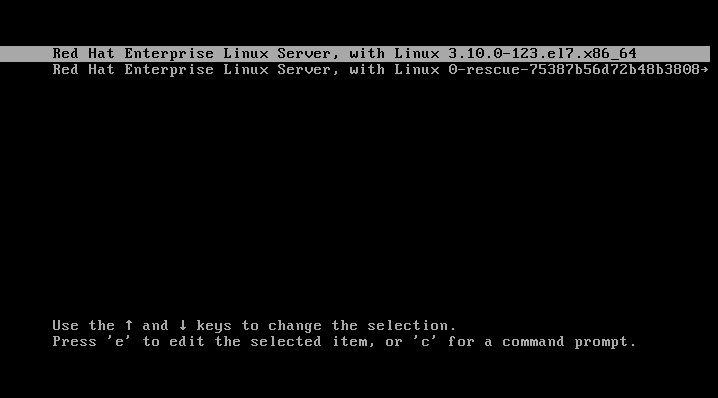
\includegraphics[width=0.45\textwidth]{root_recover00.png}
\caption{Menú de arranque grub.}
\label{fig:rootrecover:00}
\end{figure}

Ahora veremos una pantalla similar a la mostrada en la figura \ref{fig:rootrecover:01}, la cual variará según la resolución de pantalla y la configuración por defecto para la resolución en el grub. Nos desplazamos hacia abajo hasta encontrar la línea que contenga "rhgb quiet" como se muestra en la figura \ref{fig:rootrecover:02}. Estas opciones las reemplazaremos por init=/bin/bash como se muestra en la figura \ref{fig:rootrecover:03} y luego presionamos ctrl+x para arrancar el sistema.

\begin{figure}[H]
\centering
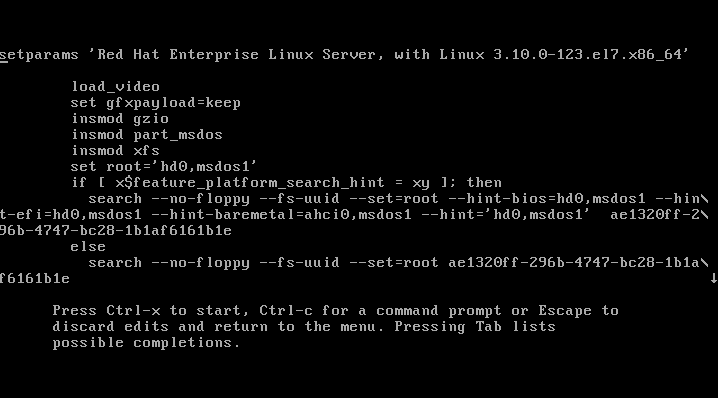
\includegraphics[width=0.45\textwidth]{root_recover01.png}
\caption{Vista inicial de opciones de arranque.}
\label{fig:rootrecover:01}
\end{figure}

\begin{figure}[H]
\centering
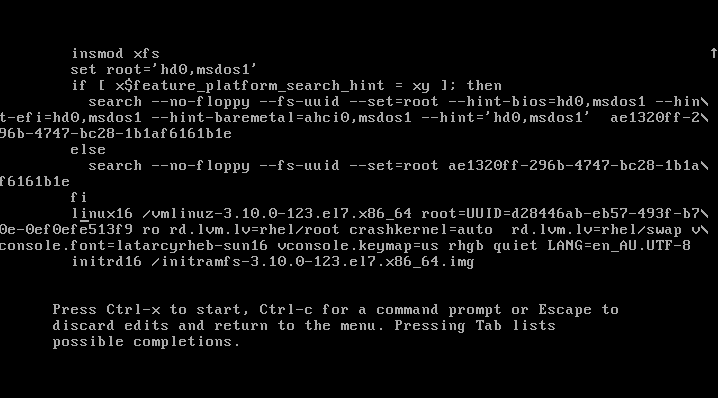
\includegraphics[width=0.45\textwidth]{root_recover02.png}
\caption{Línea con los parámetros rhgb quiet a reemplazar.}
\label{fig:rootrecover:02}
\end{figure}

\begin{figure}[H]
\centering
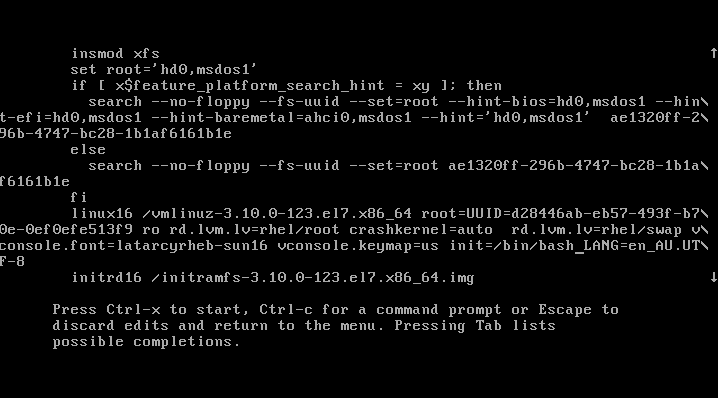
\includegraphics[width=0.45\textwidth]{root_recover03.png}
\caption{Parámetros de arranque debidamente modificados, reemplazando rhgb quiet por init=/bin/bash.}
\label{fig:rootrecover:03}
\end{figure}
Si todo transcurre con normalidad, el sistema iniciará y de una vez nos dará un prompt con acceso a root sin necesidad de contraseña alguna. Una vez acá, hacemos lo siguiente:

\begin{lstlisting} 
mount -o remount,rw /
passwd
touch /.autorelabel
exec /sbin/init
\end{lstlisting}

Lo que hicimos fue montar la partición / con opciones de lectura y escritura, para luego cambiar la contraseña por una nueva conocida mediante el comando passwd. Posteriormente, debido al funcionamiento de SELinux, se debe renombrar todo el sistema de archivos para que el cambio de contraseña tenga efecto, para lo cual se crea un archivo vacío /.autorelabel. Finalmente, reiniciamos el sistema con el comando exec /sbin/init.

\section{Sincronizar hora de los nodos mediante NTP}
En el meta nodo se encuentra instalado y corriendo un servidor NTP (Network Time Protocol) el cual se encarga de mantener sincronizada la hora y la fecha de los nodos de Cadejos. Cuando se agrega equipo nuevo al clúster, es necesario mantener esta sincronización. Para lograrlo, hacemos lo siguiente \cite{ntpclient}:

\begin{lstlisting} 
yum -y install ntp
ntpdate meta.cnca
nano /etc/ntp.conf
\end{lstlisting}

En el archivo de configuración, comentamos las líneas de comienzan con server y agregamos las siguientes:

\begin{lstlisting} 
server meta.cnca iburst
server pool.ntp.org
\end{lstlisting}

Salvamos el archivo y procedemos a hacer lo siguiente:

\begin{lstlisting} 
systemctl enable ntpd.service
systemctl start ntpd.service
\end{lstlisting}

\section{Ajuste en configuración de servidor SSH para prevenir desconexiones repentinas}
El funcionamiento de la comunicación por SSH permite el cifrado y manipulación segura de datos y funciones de manera remota. Sin embargo, hay ocasiones en las que la comunicación puede verse interrumpida, ya sea por dificultades del lado del proveedor de servicios de internet o porque la conexión se ha visto comprometida de alguna forma a nivel de seguridad, o incluso por un tema de inactividad. Este último caso es posible prevenirlo a nivel del cliente y del servidor para evitar el siguiente error \cite{brokenpipe}:

\begin{lstlisting} 
packet_write_wait: Connection to 163.178.80.34 port 22: Broken pipe
\end{lstlisting}

\subsection{Ajuste de sshd\_config en el servidor}
Este ajuste debe realizarse en todos los nodos de login disponibles en el clúster. Simplemente procedemos a abrir el archivo /etc/ssh/sshd\_config, descomentamos la siguiente línea y asignamos un tiempo a discreción:

\begin{lstlisting} 
ClientAliveInterval 60 # 60 es el valor actual. Retocar en caso de ser necesario
\end{lstlisting}

Salvamos el archivo y reiniciamos el servicio.

\begin{lstlisting} 
systemctl restart sshd.service
\end{lstlisting}

\subsection{Ajuste de ssh\_config en el cliente}
Es posible que independientemente de lo que se haga en el servidor, el cliente siga teniendo problemas para mantener la conexión activa. Para poder prevenir este problema, se debe editar el archivo /etc/ssh/ssh\_config y agregamos la siguiente línea bajo la sección Host *:

\begin{lstlisting} 
Host *
ServerAliveInterval 120 # Línea a agregar. Definir el intervalo a discreción
\end{lstlisting}

Se reinicia el servicio del lado del cliente y listo (varía de acuerdo a la distribución del cliente):

\begin{lstlisting} 
systemctl restart sshd.service
\end{lstlisting}

\clearpage